\documentclass[letterpaper,journal,twoside]{IEEEtran}
\usepackage{amsmath,amsfonts}
\usepackage{array}
\usepackage{textcomp}
\usepackage{stfloats}
\usepackage{url}
\usepackage{verbatim}
\usepackage{graphicx}
\usepackage{cite}
\usepackage{xcolor}
\usepackage{subcaption}
\usepackage{mathtools}  
\usepackage{amssymb}
\usepackage{tabulary}
\usepackage{booktabs}
\usepackage[ruled,linesnumbered]{algorithm2e}
\usepackage{algorithmic}
\usepackage{hyperref}
\usepackage{setspace}

% usepackage from 
\usepackage{adjustbox}
\usepackage{physics}
\usepackage{amsmath}
\usepackage{tikz}
\usepackage{mathdots}
\usepackage{yhmath}
\usepackage{cancel}
\usepackage{color}
\usepackage{siunitx}
\usepackage{array}
\usepackage{multirow}
\usepackage{amssymb}
\usepackage{gensymb}
\usepackage{tabularx}
\usepackage{extarrows}
\usepackage{booktabs}
\usetikzlibrary{fadings}
\usetikzlibrary{patterns}
\usetikzlibrary{shadows.blur}
\usetikzlibrary{shapes}


\newcommand{\B}[1]{\boldsymbol{#1}}
\newcommand{\TB}[1]{\textbf{#1}}
\newcommand{\etal}{\textit{et al}.~}
\newcommand{\robotConfig}{\mathcal{C}}

\begin{document}

\title{Multi-drone Motion Planning \& Control in Dynamic Environments based on Deep Reinforcement Learning}

\author{
  \IEEEauthorblockN{
    Baozhe Zhang
  }
}

\maketitle

\begingroup
\renewcommand\thefootnote{}
\footnotetext{Baozhe Zhang is with School of Science and Engineering, 
The Chinese University of Hong Kong, Shenzhen, China. 
Email: \texttt{\{baozhezhang\}@link.cuhk.edu.cn}.
Baozhe Zhang is advised by Dr.~Tin Lun Lam and 
Dr.~Yuan Gao.}
\endgroup

% The paper headers
\markboth{ERG4901: Capstone Project -- Mid-Term Report}%
%{Shell \MakeLowercase{\textit{et al.}}: A Sample Article Using IEEEtran.cls for IEEE Journals}
{Zhang: Multi-drone Motion Planning \& Control}

% \IEEEpubid{\copyright~2023 Baozhe Zhang}
% Remember, if you use this you must call \IEEEpubidadjcol in the second
% column for its text to clear the IEEEpubid mark.


\begin{abstract}
  Micro aerial vehicles (MAVs) or unmanned aerial vehicles (UAVs), popularly referred to as drones, have seen an upsurge in applications across diverse industries. Their rising prominence is also due to the need for multi-drone operations in dynamic environments, posing significant challenges in navigation and coordination. While traditional motion planning and control algorithms have achieved notable milestones, they are often constrained by system complexity, modeling limitations, and lack of generalizability. This report highlights the potential of Deep Reinforcement Learning (DRL) as an alternative approach. With its capabilities for end-to-end training, scalability, data-driven modeling, and task generalization, DRL presents a promising avenue to overcome traditional limitations. Specifically, we aim to harness DRL's potential to enable a quadrotor team to navigate through a combination of static and dynamic gates, emphasizing efficiency and score optimization. The exploration encapsulates DRL's promise in navigating advanced robotic challenges in contemporary dynamic environments.
\end{abstract}

\begin{IEEEkeywords}
  Multi-robot System, Quadrotor, Motion Planning, Control, 
  Obstacle Avoidance, Deep Reinforcement Learning
\end{IEEEkeywords}

\section{Introduction}
\IEEEPARstart{R}{ecently}, micro aerial vehicles (MAVs) or 
unmanned Aerial Vehicles (UAVs), commonly known as drones, 
have emerged as a powerful tool in various industries, 
ranging from agriculture and real estate to filmography and delivery 
services. 
Their versatility and cost-effectiveness have led to a 
surge in applications that require multiple drones to operate 
collaboratively. 
Operating in real-world dynamic environments, 
these multi-drone systems need to navigate a wide range of 
challenges, 
including moving obstacles, inter-drone coordination, and 
real-time adaptability. 
Traditional motion planning and control algorithms often  
struggle when faced with the unpredictability and complexity of such 
scenarios.

The traditional planning and control pipelines for robots' 
autonomous navigation have been extensively studied in recent
decades in the literature. 
Many complete systems with simultaneous localization 
and mapping (SLAM) and hierarchical 
planning and control frameworks can achieve outstanding 
autonomy.
For example, \cite{zhou2019robust} proposes a robust and efficient 
quadrotor motion planning system for fast flight in 
three-dimensional complex environments.
\cite{quan2023robust} introduces a distributed motion planning 
trajectory optimization framework for large-scale quadrotor 
formation flight in dense environments.
Although traditional methods can achieve impressive performance, 
there are limitations and challenges associated with these methods: 
\begin{itemize}
  \item \TB{Complexity}. The hierarchical planning and control 
  methods consist of multiple layers of modules,   
  each of which requires fine-tuning of 
  its parameters, increasing the overall complexity of the system.
  \item \TB{Modeling Limitation}. Traditional methods rely on 
  accurate models of the environment and the system. However, 
  creating precise models, especially for complex systems like 
  drones, can be challenging. Small discrepancies between the 
  model and reality can lead to significant performance 
  degradation. 
  \item \TB{Generalizability}. Many traditional methods are 
  tailored to specific tasks, environments, 
  or robot platforms. Transferring them 
  to new tasks or settings often requires significant 
  modifications. 
\end{itemize}

The capability of the 
classical hierarchical motion planning framework is 
challenged 
as the complexity and randomness of robot application 
scenarios increase. 
Recent advancements in artificial intelligence have fostered 
the development of Deep Reinforcement Learning (DRL) - a branch 
of machine learning that trains agents to make sequential 
decisions by interacting with an environment. DRL has shown 
promise in addressing complex problems in robotics 
due to its ability to learn from large 
amounts of data and adapt to changes in real-time
\cite{lee2020learning,hwangbo2017control,gu2017deep}.
DRL-based motion planning and control bring insights to 
overcome the challenges faced by traditional methods: 
\begin{itemize}
  \item \TB{Unified framework}. DRL allows for unified end-to-end 
  training and inference where planning and control can be 
  learned 
  jointly, potentially leading to more cohesive and optimal 
  solutions.
  \item \TB{Scalability with multiple agents}.  DRL can be 
  extended to multi-agent scenarios using techniques like 
  multi-agent reinforcement learning, enabling cooperative or 
  competitive behaviors among agents.
  \item \TB{Data-driven model}. Unlike model-based methods which 
  require precise system models, DRL can learn planning and  
  control policies directly from interaction data, potentially  
  avoiding modeling inaccuracies.
  \item \TB{Generalization}. Since many DRL methods are 
  model-free, the training can be generalized to different 
  robot platforms and even to many other tasks by changing 
  the reward functions defined in DRL algorithms.
\end{itemize}


Traditional motion planning and control methods have long 
provided 
reliable solutions in robotics. 
However, their limitation emerge with the increasing complexity of tasks, 
such as 
navigating in dynamic and stochastic environments.
In this report, we propose to address these limitations
by utilizing the 
adaptability of DRL.  
We aim to guide a quadrotor team through a mix of static 
and dynamic gates, striving for maximum scores in minimal time. 
This task will demonstrate the potential of DRL in advanced 
robotic navigation challenges.



\section{Related Work}

In this section, we will investigate both traditional 
and DRL-based methods for planning and control in the 
literature, with a focus on aerial systems 
such as drones or quadrotors.

Traditional planning and control frameworks are decoupled.
The path-planning (or motion-planning) module serves as a guide system 
for the low-level controller driving the robot's movement. 
This module needs to generate a geometrically 
collision-free and possibly kinodynamically feasible trajectory 
(or motion setpoints) for the low-level controller.
Then the low-level control module can use these motion 
setpoints to control the actuators on the robots to move.
Recent DRL-based methods attempt to combine these two modules 
into a coupled system through repeated learning. 
The robots learn to navigate themselves through trials and learning 
from the environments.
These trials are mainly conducted in simulations, 
where high-fidelity physics engines are required. 
By utilizing certain DRL training methods, 
the trained models (e.g., neural networks) can be deployed 
on real robots for autonomous navigation in various static 
or dynamic environments.

\subsection{Configuration Space and Map Representation}
The configuration space (C-Space) contains all possible transformations
for robots. 
For a robot with $n$ degrees of freedom, the set of 
transformations, which is a manifold with dimension $n$, is 
the configuration space for that robot, denoted by $\robotConfig$
\cite{quan2020survey}. 
For example, the C-Space for the 2D rigid body is $SE(2)$ 
and for the 3D rigid body is $SE(3)$.
The obstacle region $\robotConfig_{\text{obs}} \subseteq \robotConfig$ 
represents the transformations where the robot collide with the obstacles. 
The free space is defined as $\robotConfig_{\text{free}} = 
\robotConfig \backslash \robotConfig_{\text{obs}}$.
Therefore, the motion planning problem can be formulated as 
finding a path 
$
  \tau : \left[0,1\right]\rightarrow \robotConfig_{\text{free}}
$
such that $\tau(0) = q_{\text{start}} 
\in \robotConfig_{\text{free}}$ and 
$\tau(1) = q_{\text{goal}} \in \robotConfig_{\text{free}}$
are the start and goal transformations, respectively.

Although mapping techniques are typically associated 
with the problem of SLAM, mapping with
known poses of the robot is also important. 
Many motion planning algorithms rely on given maps. 
One commonly used map representations is occupancy 
grid map \cite{elfes2013occupancy}, which divides the space
into cells (2D or 3D) that store the probabilistic estimate of the 
states (occupied or not).
Efficient data structures can be used to 
represent the space. 
The K-Dimensional Tree (K-D Tree) is an efficient data
structure that organizes multi-dimensional point data 
\cite{bentley1975multidimensional}
enabling fast search of nearest neighbors.
The Incremental K-D Tree (ikd-tree) \cite{cai2021ikd} 
incrementally updates the K-D tree with only new points.
Octomap \cite{wurm2010octomap} based on octrees using 
probabilistic occupancy estimation proposes a compact 
data structure for map representation.
Another approach for volumetric representation is based on 
signed distance fields (SDFs) \cite{curless1996volumetric}
as introduced in the computer graphics literature.
In recent robotic applications, \cite{lin2018autonomous} uses
truncated signed distance fields (TSDFs)
\footnote{The TSDF of a voxel is defined as the nearest 
distance to the surrounding surface in a truncation distance. 
If the voxel is between the robot and the surface, 
the value is positive, negative otherwise. }
to reconstruct surfaces around the MAV. 
\cite{oleynikova2017voxblox} and later \cite{han2019fiesta}
use Euclidean signed distance fields (ESDFs) to incrementally
update the voxel map with distance and gradient information, 
which is convenient for gradient-based trajectory optimization.

\subsection{Traditional Planning and Control}

\begin{figure}[h]
  \centering
  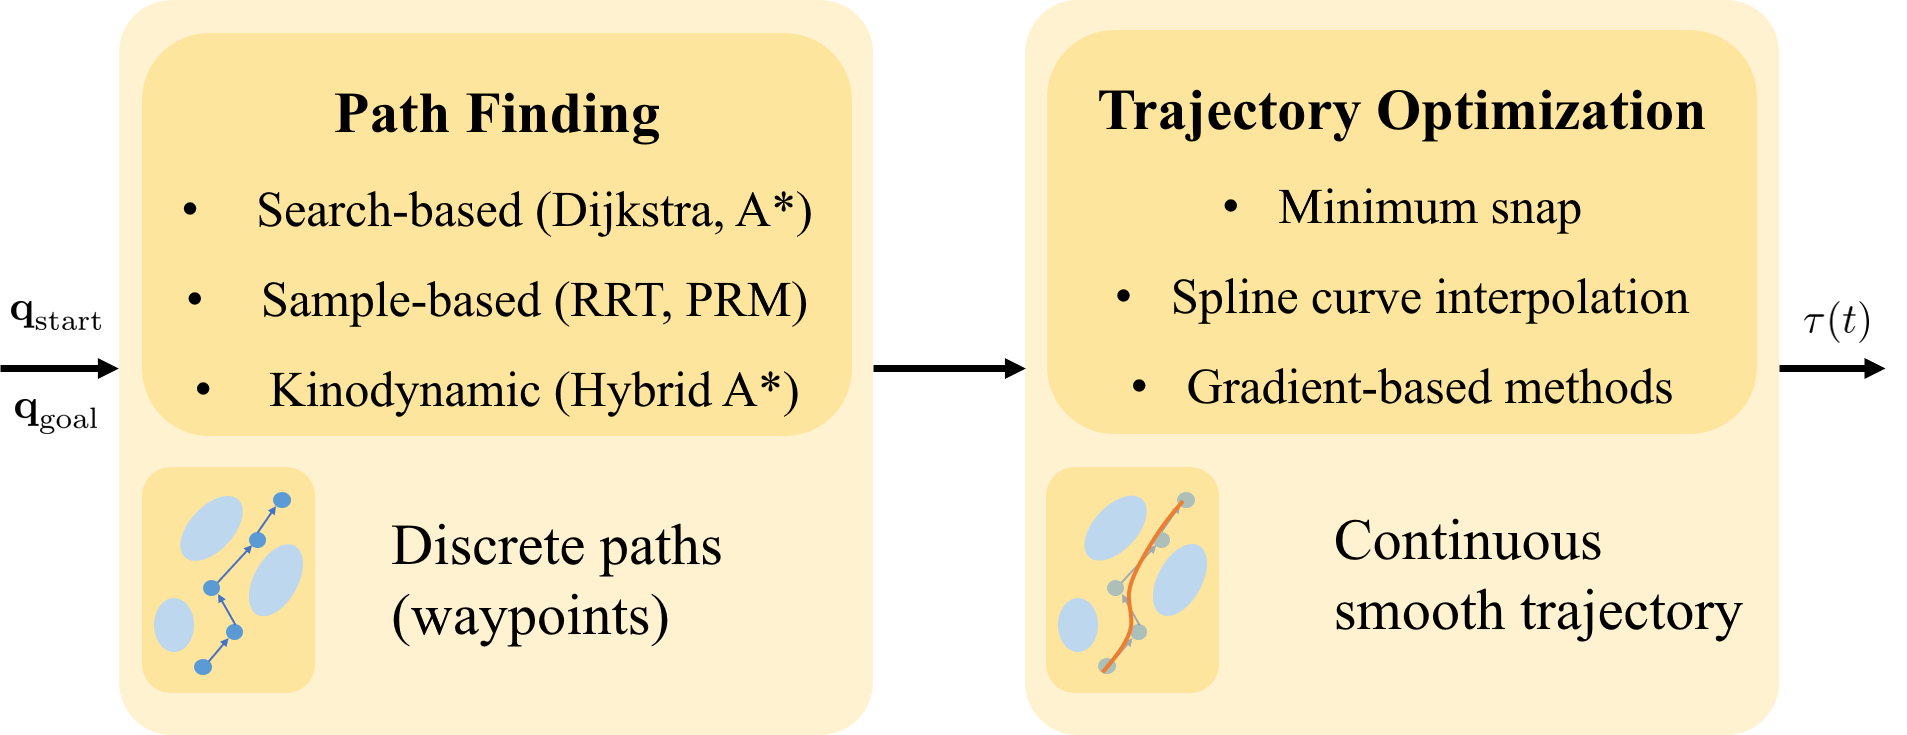
\includegraphics[width=.5\textwidth]
  {../figures/frontback.png}
  \label{fig:concept}
  \caption{Hierarchical planning pipeline: The path-finding module 
finds a geometric collision-free path, and then trajectory
optimization module generates a continuous state-admissable and kinodynamically
feasible trajectory.}
\end{figure}
In general, path-planning algorithms for robot navigation 
can be divided into two major categories: 
global and local methods.
\footnote{The distinction between global and local
planning methods is not strict, as high-frequency global 
re-planning can eliminate the need for local path planning.}  
Global methods focus on finding collision-free paths from 
the current robot position to a global goal position in mostly 
static scenes, while local methods tend to reactively 
avoid both static and dynamic obstacles and they are usually coupled with control modules. 
To generate smooth trajectories for robots to 
follow based on discrete planned waypoints, the 
trajectory optimization module is usually added to 
the pipeline. 
In the literature, the path-finding module 
is called the frontend and the 
trajectory-optimization module is called the backend. 
A typical hierarchical planning pipeline can be 
found in Fig.~\ref{fig:concept}.

\subsubsection{Path Finding (Frontend)}

In the path-finding stage of global planning, 
methods can be categorized 
into three major directions: {search-based}, 
{sample-based}, and {kinodynamic} methods. 


% \begin{algorithm}
\caption{A* Algorithm}
\label{alg:a_star}
\begin{algorithmic}[1]
\REQUIRE $start$: starting node, $goal$: goal node
\STATE $openSet \gets \{start\}$
\STATE $cameFrom \gets$ empty map
\STATE $gScore[start] \gets 0$
\STATE $fScore[start] \gets heuristic(start, goal)$
\WHILE{$openSet$ is not empty}
  \STATE $current \gets$ node in $openSet$ with lowest $fScore$
  \IF{$current = goal$}
    \RETURN reconstructPath($cameFrom$, $current$)
  \ENDIF
  \STATE remove $current$ from $openSet$
  \FORALL{$neighbor$ of $current$}
    \STATE $tentativeGScore \gets gScore[current] + dist(current, neighbor)$
    \IF{$neighbor$ not in $gScore$ or $tentativeGScore < gScore[neighbor]$}
      \STATE $cameFrom[neighbor] \gets current$
      \STATE $gScore[neighbor] \gets tentativeGScore$
      \STATE $fScore[neighbor] \gets gScore[neighbor] + heuristic(neighbor, goal)$
      \IF{$neighbor$ not in $openSet$}
        \STATE add $neighbor$ to $openSet$
      \ENDIF
    \ENDIF
  \ENDFOR
\ENDWHILE
\RETURN failure
\end{algorithmic}
\end{algorithm}

{Search-based} algorithms such as depth-first 
search (DFS) \cite{cormen2022introduction}, 
breadth-first search (BFS) \cite{cormen2022introduction}, 
Dijkstra \cite{wang2011application}, and 
A* \cite{hart1968formal}, use graph-search methods 
with certain pre-defined heuristics to find 
geometrically feasible paths on given grid maps. 
These methods assume that 
is the map is given, which can be challenging to obtain
in certain situations. 
Although these search-based methods can perform well, they 
can have longer search times when the space scales.
% Alg.~\ref{alg:a_star} shows the A* path-planning algorithm which returns the shortest path from the source node to the target node. 
{Sample-based} methods such as rapidly exploring random 
tree (RRT), probabilistic roadmap (PRM), and their 
variants (e.g., RRT* and PRM*) use sampling in C-Space 
to create collision-free paths \cite{lavalle2001rapidly,
karaman2011sampling,kavraki1996probabilistic}. 
% The general form of RRT algorithm can be found in 
% Alg.~\ref{alg:rrt}.
% \begin{algorithm}
\SetAlgoLined
\KwIn{Start state $q_{start}$, goal region $G$, maximum number of iterations $K$, step size $\Delta q$, collision checking function $IsCollisionFree$, tree $T$}
\KwOut{A path from $q_{start}$ to $G$ if found, otherwise failure}
Add $q_{start}$ to $T$\;
\For{$k=1$ \KwTo $K$}{
  $q_{rand} \gets$ RandomState()\;
  $q_{near} \gets$ NearestVertex($T$, $q_{rand}$)\;
  $q_{new} \gets$ Steer($q_{near}$, $q_{rand}$, $\Delta q$)\;
  \If{!IsCollisionFree($q_{near}$, $q_{new}$)}{
    continue\;
  }
  Add $q_{new}$ to $T$\;
  \If{$q_{new} \in G$}{
    \Return Path($q_{start}$, $q_{new}$)\;
  }
}
\Return failure\;
\caption{Rapidly-Exploring Random Tree (RRT)}
\label{alg:rrt}
\end{algorithm}

However, the tree nodes in these methods need to cover the 
whole C-Space which may result in heavy computational 
loads especially when the space is large.  

Both search- and sample-based methods can generate 
geometrically collision-free paths but they may be jerky
\footnote{Jerk $\B{j}$ is the third time-derivative 
of the position $\B{p}$} or 
violate the underlying robots' dynamics.
For example, most ground vehicles are not 
holonomic, i.e., they cannot move freely in all directions 
in 2D space. Instead, their motions are governed by  
mechanical and motion constraints, such as velocities and 
accelerations.
To account for both the kinematic and dynamic 
constraints of specific
robot platforms and reduce the stress on the backend 
optimization part, {kinodynamic} methods are introduced
in the literature. 
Donald \etal \cite{donald1993kinodynamic} first proposed 
the term {kinodynamic} motion planning.
The authors presented the first provably good approximation 
algorithm for motion planning
in 2D and 3D environments with polyhedral obstacles.
The state-lattice method \cite{pivtoraiko2011kinodynamic} is also 
used for kinodynamic motion 
planning, where the boundary value problem (BVP) needs to be 
solved to obtain the corresponding control inputs 
for the sampled states. 
In \cite{zhou2019robust}, the authors propose a method that
samples in the control space to generate possible motion 
primitives, and then 
search and select kinodynamically
feasible paths based on these motions. 
Webb and Berg \cite{webb2013kinodynamic} propose the
kinodynamic RRT* method, which generalizes the
earlier work on RRT* \cite{karaman2011sampling} for kinodynamic 
systems. This method guarantees asymptotic optimality for 
any system with controllable linear
dynamics in state spaces of any dimension.
\cite{dolgov2008practical,dolgov2009autonomous,dolgov2010path}
propose the hybrid A* (or hybrid-state A*) algorithm, which 
extends the original A* algorithm for kinodynamic graph searching.

Another less common method such as model predictive 
control (MPC) added with obstacle constraints or with 
additional environment-related 
terms \cite{park2009obstacle,ji2016path}  can also be 
used to generate collision-free paths. This method is based on 
quadratic-programming (QP) optimization. 
However, MPC-related methods need to balance the 
length of the time horizon, computational loads, and 
optimality. A short time horizon often leads to 
sub-optimal solutions for the problem.




\subsubsection{Trajectory Generation and Optimization (Backend)}
Most path-finding algorithms only generate geometric 
feasible paths, without any time information. 
The goal of trajectory generation and optimization is to 
provide both spatial and temporal profiles based on the 
found paths \cite{quan2020survey}. 
Essentially, the trajectory is a geometric path parametrized 
in time, with guaranteed kinodynamic feasibility and smoothness.
Usually, it is optimized with goals such as minimizing the 
total ``energy'' spent along the path while satisfying the 
kinodynamic constraints of the robots.
Mellinger and Kumar \cite{mellinger2011minimum} propose 
a minimum snap trajectory generation method based on the 
differential flat property of quadrotor or multirotor 
systems. 
This method uses QP optimization with 
hard constraints for flight corridors to generate optimal 
trajectories. 
Among the prevalent methods in the literature are 
interpolating curves \cite{dong2023review}.
Zhou \etal \cite{zhou2019robust} propose a trajectory 
optimization method based on the convex hull property of 
B-splines and provide a time adjustment method for it.
Wang \etal \cite{wang2022geometrically} propose a 
minimum-control (MINCO) trajectory family based on 
multi-degree polynomials that can be 
optimized with user-defined state-input constraints for 
multi-copter motion planning.
Gradient-based methods such as
CHOMP \cite{ratliff2009chomp} and 
EGO-Planner \cite{zhou2020ego} are also popular methods 
for trajectory optimization.

\subsubsection{Local Methods}
Most global methods perform well in static environments, 
but poorly in dynamic environments. 
Local path-planning methods can be employed to handle 
this problem. 
An early local obstacle-avoidance method is artificial 
potential field (APF) \cite{warren1989global}.
APF formulates the potentials on a given path as the 
inside and outside ones, and pushes the path from the
high-potential to the low-potential region by finding the 
lowest potential value. 
If the waypoints on the path cross the 
obstacle (inside the obstacle), the potential is formulated as 
\[
U_{\text{in}} = 
U_{\text{max}}\left(1 - \frac{R_{\text{in}}}{R_{\text{max}}}\right) + 
U_{\text{offset}}
\]
where $U_{\text{max}}$ is the max potential, 
$R_{\text{in}}$ is the distance to the centroid of the 
obstacle, $R_{\text{max}}$ is the max radius of the 
obstacle, and $U_{\text{offset}}$ is the extra 
potential penalty.
The outside potential is formulated as 
\[
U_{\text{out}} = 
\frac{1}{2}U_{\text{offset}}\left(1+ \frac{1}{1+R_\text{out}}\right)
\]
where $R_{\text{out}}$ is the distance outside the obstacle.
APF can be used for quadrotor path-planning \cite{chen2016uav}.
However, when multiple obstacles are present, APF can suffer 
from the problem of local minimum \cite{koren1991potential}.
The dynamic window approach (DWA) \cite{seder2007dynamic} can 
be used for dynamic obstacle avoidance, where DWA considers
the kinodynamic feasibility of the robot and samples in the 
velocity space to generate motion primitives for collision 
avoidance. 
The idea of velocity obstacle (VO) is proposed and generalized
by Van Den Berg \cite{van2011reciprocal,van2011reciprocal2,bareiss2013reciprocal}.
Reciprocal VO-based obstacle avoidance methods can be used
for motion planning for robots.  
However, the smoothness of the generated paths cannot be 
guaranteed. 
Dynamical system modulation (DSM)
\cite{khansari2012dynamical,huber2022fast,huber2023avoidance}
is another approach to achieve obstacle avoidance for local
motion planning, which directly changes the first-order 
linear system of the robot (point-mass model) to guide the 
robot away from the obstacle by adding a linear transformation
(obtained from the environment) to the initial velocity of 
the robot.
However, the algorithms are limited with star-shaped obstacles, 
and the performance of DSM on agile robots such as quadrotors
is still skeptical.

\subsubsection{Control}
The control module is usually responsible for trajectory 
tracking (TT) tasks for planning and control.
Despite the low-level controllers of the actuators of the 
robots, which track the setpoints of torques, angular 
velocities, or accelerations, the controllers used in the TT
phase focus on designing controllers based on system
equations so that robots can track a given reference 
trajectory asymptotically. 
\cite{majd2019stable} proposes using the input-output 
linearization technique to optimize the tracking error for
car-like robot trajectory tracking.
MPC or receding horizon control (RHC)
is also a popular method to perform TT via optimization.
\cite{kunhe2005mobile} used non-linear MPC to control the 
wheeled robots for TT.
\cite{romero2022model,ji2021cmpcc} propose model predictive
contouring control (MPCC) by adding the time profile to the 
controller design to minimize the traversal time while tracking
the reference trajectory.
Thanks to the flexibility of the framework of MPC, the model 
can be reformulated to satisfy different needs. 
In \cite{zhang2023coni}, the authors propose cooperative 
non-inertial frame based model predictive control (CoNi-MPC), 
which directly formulates the quadrotor model in a target's 
body non-inertial frame and controls the quadrotor tracking 
trajectories predefined in the target's frame.

\subsection{DRL-based Planning and Control}
DRL, which combines deep learning 
and reinforcement learning (RL), 
has become increasingly popular in the field of motion planning 
and control. 
Its adaptability, ability to learn from raw data, and scalability 
have made it an attractive choice for researchers.
For instance, Mnih \etal introduced the deep Q network (DQN), 
a DRL algorithm capable of achieving human-level performance in various video games \cite{mnih2015human}. 
This breakthrough has established a precedent for applying 
DQN in motion planning and control for robots. 
Additionally, Lillicrap \etal went on to expand the 
capabilities of DQN by proposing the deep deterministic policy 
gradient (DDPG) algorithm. 
This algorithm facilitates learning policies in continuous action 
spaces, a necessary feature for most real-world control tasks 
\cite{lillicrap2015continuous}.

In the context of aerial vehicles, Zhang \etal integrated MPC with DRL. 
They demonstrated the combination through guided policy search 
with an MPC controller in simulation. 
Their work employed a policy that maps raw sensor data to rotor 
velocities to achieve obstacle avoidance \cite{zhang2016learning}. 
Moreover, Kahn \etal proposed a DRL methodology that excelled in 
navigation tasks using raw monocular camera images \cite{kahn2018self}.

The application of DRL in drone racing and agile flight dynamics 
has received significant attention in recent studies \cite{loquercio2019deep, song2021autonomous, song2022policy, penicka2022learning, song2023reaching}. 
These studies highlight the effectiveness of DRL in motion 
planning and control, particularly in addressing the demands of 
high-speed agile navigation for quadrotors.


\section{Problem Formulation}

\subsection{Quadrotor Dynamics}
The quadrotor used in the task is modeled as a six degree-of-
freedom rigid body with mass $m$ and diagonal moment of 
inertial matrix $\B{J}$.
The dynamics of the system can be formulates as: 
\begin{equation}
\label{eq:quadrotor_system}
\begin{aligned}
  \dot{\B{p}} &= \B{v}
  \\  
  \dot{\B{v}} &= {}^W\B{q}_B \odot {}^B\B{c} + \B{g}
  \\
  {}^W\dot{\B{q}}_B &= \frac{1}{2} {}^W\B{q}_B \odot {}^B\B{\omega}
  \\
  {}^B\dot{\B{\omega}} &= 
  \B{J}^{-1}({}^B\B{\eta} - {}^B\B{\omega} \times \B{J}{}^B\B{\omega})
\end{aligned}
\end{equation}
where $\B{p}$ and $\B{v}$ are the position and velocity 
vectors in the world frame $W$. 
We use a unit quaternion 
${}^W\B{q}_B = \left[q_w, q_x, q_y, q_z\right]^\top$ 
to represent the rotation transformation from body frame 
$B$ to world frame $W$
and 
${}^B\omega = \left[\omega_x, \omega_y, \omega_z\right]^\top$ to denote the angular velocity (body rates) in the 
body frame $B$.
The gravity vector $\B{g}$ is $\left[0,0,-g_z\right]$ where
$g_z$ is $9.81\;\text{m}\;\text{s}^{-2}$.
Finally, $\B{c} = \left[0,0,c\right]$ is the collective 
mass-normalized thrust in the body frame $B$. 
The conversion of single rotor thrusts 
$\left[f_1, f_2, f_3, f_4\right]$ to 
mass-normalized thrust $c$ 
and body torques ${}^B\B{\eta}$ is formulated as
\[
  c = \frac{1}{m}\sum_{i=1}^4 f_i,\;
  {}^B\B{\eta} = 
  \begin{bmatrix}
    l/\sqrt{2}(f_1 - f_2 - f_3 + f_4) \\
    l/\sqrt{2}(-f_1 - f_2 + f_3 + f_4) \\
    \kappa(f_1 - f_2 + f_3 - f_4)
  \end{bmatrix}
\]
where $l$ is the arm length and $\kappa$ is the torque 
constant.
For each motor force $f_i$, it is modeled as 
$f_i = \alpha \omega_i^2$, where $\alpha$ is the motor 
force constant and $\omega_i$ is the motor's rotation speed
(rad/s).
The full state of the quadrotor is defined as 
$\B{x} = \left[\B{p}, \B{v}, {}^W{\B{q}}_B, 
{}^B\B{\omega}\right]^\top$ and the input as 
$\B{u} = \left[\omega_1, \omega_2, \omega_3, 
\omega_4\right]^\top$.

\subsection{Task Formulation}

The primary objective of our quadrotor team is to traverse a 
complex environment, transitioning through as many static and 
dynamic gates as possible, initiating from the start position 
$ \B{p}_{\text{start}} $ and ending at the goal position 
$ \B{p}_{\text{goal}} $, all within a minimal flight time. 
Given that we are working with $ N $ quadrotors and $ M $ 
gates, 
each gate's position and orientation can be delineated as 
$ \B{p}_i $
and $ \B{q}_i $respectively. 
This task underscores a delicate balance: 
the quadrotor team must navigate between 
exploration (to identify and target potential gates)
and exploitation, 
ensuring that they traverse the maximum number of gates while 
rapidly progressing towards $ \B{p}_{\text{goal}} $.
Mathematically, given $N$ quadrotors, $M$ gates 
with poses $\left\{(\B{p}_1,\B{q}_i), \dots, 
(\B{p}_M, \B{q}_M)\right\} 
\subset \mathbb{R}^3\times\mathbb{S}^3$, we can 
formulate the problem in a general optimization form:
\begin{equation}
  \label{eq:general_opt}
  \begin{aligned}
    \max \quad & G \\
    \textrm{s.t.} \quad & \min \quad T \\
    & \B{p}^{(i)}(0) = \B{p}_\text{start} \quad i = 1\dots N \\
    & \B{p}^{(i)}(T) = \B{p}_\text{end} \quad i = 1\dots N \\
    & G \le M \\
    & T \ge 0
  \end{aligned}
\end{equation}
where $G$ represents the number of gates traversed by the 
quadrotor team, $T$ is the time taken for the team moving
from the initial to the goal position, and $\B{p}^{(i)}$ 
is the position of the $i^{\text{th}}$ quadrotor in the 
team. 

To address this complex navigation challenge, we employ a 
DRL-based approach. 
This method stands apart from traditional planning algorithms, 
offering a blend of data-driven adaptability with strategic 
control, tailor-made for dynamic environments.
The DRL model would receive the environmental state, encompassing 
the positions of static and dynamic gates, quadrotor's current 
position, and other potential obstacles. 
Based on this, the model would decide the next best action to move closer to the goal 
while maximizing the number of gate traversals and minimizing the 
total time.



\bibliographystyle{IEEEtran}
\bibliography{report}


\end{document}


